\section{Режимы аутентифицированного шифрования. Современные стандартизированные решения.}

Аутентифицированное шифрование позволяет обеспечить не только конфиденциальность данных, но и их аутентичность. 

Есть два варианта: использовать одну из комбинаций имитовставки и шифрования, либо специальный режим шифрования. 

\subsection{Имитовставка + шифрование}

Комбинировать имитовставку и шифрование можно одним из следующих трёх способов:

\begin{enumerate}
	\item Encrypt-and-MAC: открытый текст отдельно зашифровывается и для него отдельно вырабатывается имитовставка, т.е. сторона передаёт сообщение вида $E(m), MAC(m)$, где $E$ -- зашифрование сообщения, $MAC$ -- получение имитовставки для сообщения, $m$ -- открытый текст. 
	\item MAC-then-encrypt: сначала вычисляется имитовставка для открытого текста, присоединяется к открытому тексту (конкатенацией), а потом полученное сообщение зашифровывается, т.е. сторона передаёт сообщение вида $E(m || MAC(m))$, где $||$ -- конкатенация битовых строк. 
	\item Encrypt-then-MAC: сообщение сначала зашифровывается, потом для шифртекста вырабатывается имитовставка и передаётся вместе с шифртекстом, т.е. сторона передаёт сообщение вида $E(m), MAC(E(m))$.
\end{enumerate}

Во всех трёх вариациях необходимо обязательно использовать разные ключи для имитовставки и зашифрования. В целом можно использовать любые алгоритмы выработки имитовставки и шифрования, если они сами по себе достаточно безопасны. 

Encrypt-and-MAC является наименее безопасным, т.к. имитовставка разрабатывается в первую очередь для того, чтобы её нельзя было подделать. Т.е. внимание тому, не несёт ли она какой-то информации о тексте, из которого вырабатывалась, не уделяется, т.к. она чаще всего отправляется вместе с открытым текстом. Таким образом, теоретически имитовставка может дать злоумышленнику дополнительную информацию для криптоанализа передаваемой информации. Однако этот вариант используется в SSH.

MAC-then-encrypt более безопасен, потому что в нём <<закрыта>> проблема, описанная для предыдущего варианта. Однако, чтобы понять, что сообщение повреждено, принимающей стороне необходимо сначала расшифровать повреждённых шифр текст, что занимает время, а также представляет собой уязвимость для атаки с выбранным шифртекстом (см. вопрос 24). Тем не менее, он использовался в TLS во всех версиях, кроме последней.

Encrypt-then-MAC наиболее безопасен и удобен из этих трёх подходов, потому что принимающей стороне нет необходимости расшифровывать всё сообщение, чтобы понять, что оно повреждено, достаточно проверить имитовставку. Этот вариант используется в IPSec. 

\subsection{Аутентифицированные шифры}

Аутентифицированные шифры -- то же, что обычные шифры, но в результате своей работы дают не только шифртекст, но ещё и имитовставку. Т.е. получается следующая схема: $AE(m) = (C, T)$, где $C$ -- шифртекст, $T$ -- имитовставка, $AE$ -- функция аутентифицированного зашифрования (authenticated encryption).

Соответственно, существует функция аутентифицированного расшифрования -- $AD, AD(C, T) = m$, которая возвращает ошибку в случае, если имитовставка оказалась неверной.

В современных стандартах, например, TLS 1.3, требуется не просто аутентифицированное шифрование (AE), а аутентифицированное шифрование с ассоциированными данными (AEAD). Это шифрование с аутентификацией, которое позволяет оставлять часть данных незашифрованными, но аутентифицированными. Т.е. MAC применяется ко всем, а зашифрование только к части передаваемых данных. Это нужно, например, при передаче сетевых пакетов, когда сами передаваемые данные должны быть зашифрованы и аутентифицированы, но заголовок, содержащий, например, IP-адрес назначения, должен быть аутентифицирован, но передаваться открыто. Таким образом, вводится функция зашифрования:

$AEAD(m, m_a) = (C, m_a, T)$, где $m_a$ -- дополнительные данные, которые не зашифровываются. И соответствующая ей функция расшифрования:

$ADAD(C, m_a, T) = (m, m_a)$.

Дополнительно, чтобы одни и те же открытые тексты не превращались всегда в одни и те же шифртексты, используется вектор инициализации (см. вопрос 16).

Наиболее распространённым из таких протоколов является AES-GCM. На самом деле GCM-mode может использоваться с любым симметричным шифром, но чаще всего встречается именно в связке с AES. GCM это Galois/counter mode. Называется так, потому что использует режим гаммирования (CTR -- counter) для зашифрования и умножение в поле Галуа для имитовставки. 

Принцип работы проще показать на схеме (Рис. \ref{fig:fig18-1}), которая уехала в другой вопрос. 

\begin{figure}[h]
	\centering
	
	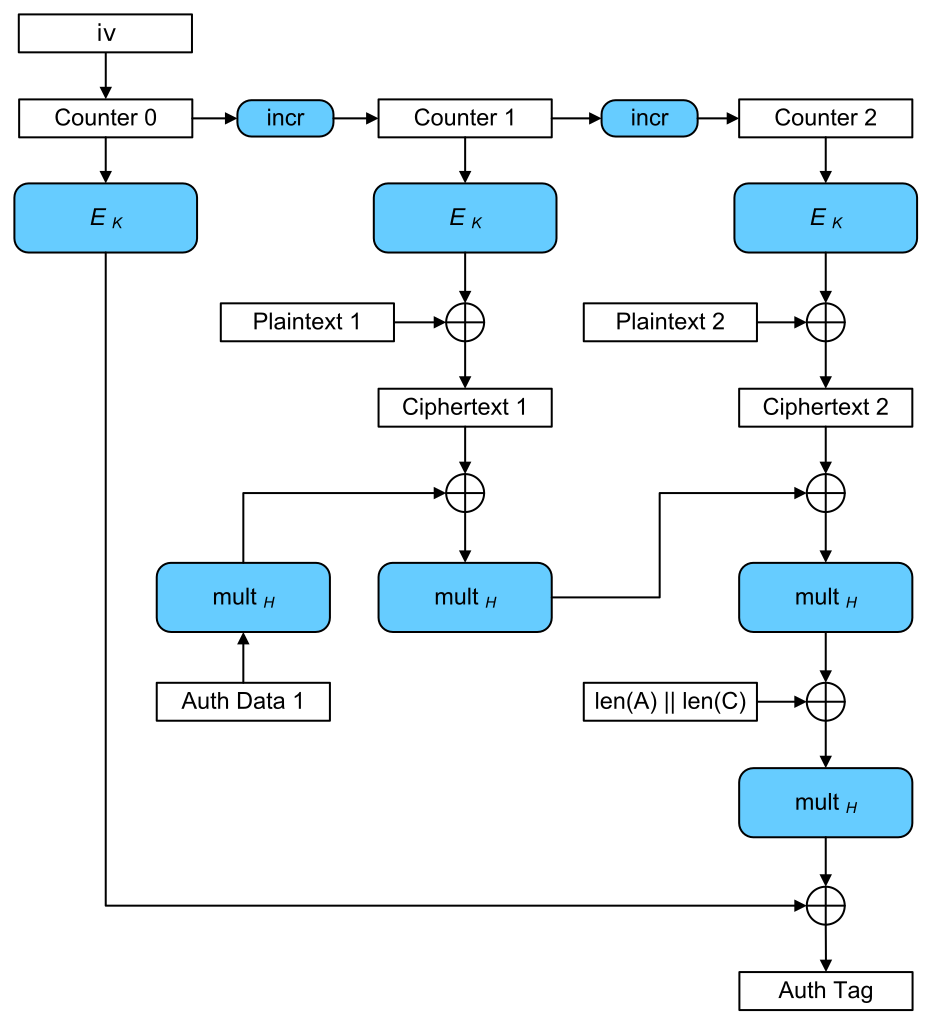
\includegraphics[width=0.8\linewidth]{Вопросы/q18-pic/AES-GCM.png}
	
	\caption{AES-GCM, к вопросу 18}
	
	\label{fig:fig18-1}
	
\end{figure}

На рисунке Auth data -- открытые данные, которые необходимо присоединить, Plaintex -- текст, который всё-таки нужно зашифровать, $mult_H$ -- операция умножения полиномов в поле Галуа, $H = E_K(0^{128})$. 

Проблемой этого алгоритма является только то, что нельзя использовать повторяющиеся инициализирующие значения. 

Помимо AES-GCM существуют и другие аутентифицированные шифры, например, OCB, SIV. 


 

